\chapter{phase transitions: criticality, universality, and scaling}
\begin{itemize}
	\item 热力学系统可以分为两类: noninteracting \& interacting.
	
	\item noninteracting 的系统包括: the specific heat of gases (section \ref{1.2} and \ref{6.4}); the specific heat of solids (section \ref{7.4}); chemical equilibrium in an ideal gas or a dilute solution (section \ref{6.5}); condensation of an ideal Bose gas (section \ref{7.1} and \ref{7.2}); spectral distribution of the blackbody radiation (section \ref{7.3}); the free electron theory of metals (section \ref{8.3}); the phenomenon of paramagnetism (section \ref{3.7} and \ref{8.2}).
	\begin{itemize}
		\item 除了 Bose--Einstein condensation 之外, 所有这些系统的 thermodynamic functions 都是光滑的.
	\end{itemize}
	
	\item interacting 的系统包括: the condensation of gases; the melting of solids; the coexistence of phases (especially near a critical point); mixtures and solutions (包括 the onset of phase separation); ferromagnetism and antiferromagnetism; the order--disorder transitions in alloys; the superfluid transition from liquid He I to liquid He II; transition from a normal to a superconducting material.
	\begin{itemize}
		\item interacting 的系统, 经常会遇到 thermodynamic functions 具有 analytic discontinuities or singularities 的情况, 相应地, 会遇到各种 phase transitions.
	\end{itemize}
\end{itemize}

\section{general remarks on the problem of condensation}
\begin{itemize}
	\item 对任何热力学系统, 都有
	\begin{equation}
		\Big( \frac{\partial P'}{\partial v} \Big)_{V, T} = - \frac{k_B T}{v^2} \frac{\braket{N}}{\braket{(\Delta N)^2}} \leq 0,
	\end{equation}
	其中 $P'$ 定义为
	\begin{equation}
		P' := \frac{k_B T}{V} \ln Z_\text{GC} \equiv - \frac{\Phi_\text{G}}{V},
	\end{equation}
	对于 homogeneous system (注意 multiphase systems 也可以是 homogeneous, 但要忽略表面效应) 有 $P' = P$.
	
	\begin{tcolorbox}[title=calculation:]
		注意到
		\begin{equation}
			- \frac{V}{N^2} \Big( \frac{\partial P'}{\partial v} \Big)_{T, V} = \Big( \frac{\partial P'}{\partial N} \Big)_{T, V} = - \frac{1}{V} \Big( \frac{\partial \Phi_\text{G}}{\partial N} \Big)_{T, V},
		\end{equation}
		且
		\begin{equation}
			\Big( \frac{\partial \Phi_\text{G}}{\partial N} \Big)_{T, V} = - N \Big( \frac{\partial \mu}{\partial N} \Big)_{T, V} = - \frac{N}{\big( \frac{\partial N}{\partial \mu} \big)_{T, V}} = - \frac{N}{\beta \braket{(\Delta N)^2}},
		\end{equation}
		最后一个等号用到了 \eqref{4.4.1}.
	\end{tcolorbox}
	
	\item 注意到, 在某些区间 $\braket{(\Delta N)^2} \sim O(N^2)$, 此时
	\begin{equation}
		\Big( \frac{\partial P'}{\partial v} \Big)_{V, T} \sim O(N^{- 1}) \simeq 0.
	\end{equation}
\end{itemize}

\section{condensation of a van der Waals gas}
\subsection{mean field estimate}
\begin{itemize}
	\item 考虑气体分子之间具有相互作用, 那么系统的 partition function 为
	\begin{align}
		Z_\text{C}(T, V, N) &= \frac{1}{N!} \int \frac{d^{3 N} p d^{3 N} q_i}{h^{3 N}} e^{- \beta \sum_{i = 1}^N \frac{p_i^2}{2 m}} e^{- \beta \sum_{i < j} u(q_i - q_j)} \notag \\
		&\simeq \frac{1}{N! \lambda^{3 N}} \Big( V - \frac{N \Omega}{2} \Big)^N e^{\beta \frac{V}{2 v^2} u}.
	\end{align}
	
	\begin{tcolorbox}[title=calculation:]
		考虑
		\begin{equation}
			\sum_{i < j} u(\vec{q}_i - \vec{q}_j) = \frac{1}{2} \int d^3 r_1 d^3 r_2 \, n(\vec{r}_1) n(\vec{r}_2) u(\vec{r}_1 - \vec{r}_2),
		\end{equation}
		其中
		\begin{equation}
			n(\vec{r}) = \sum_{i = 1}^N \delta^{(3)}(\vec{r} - \vec{q}_i) \Longrightarrow \int d^3 r \, n(\vec{r}) = N,
		\end{equation}
		作 approximation of uniform density, 那么
		\begin{equation}
			n(\vec{r}) \simeq \frac{N}{V} \Longrightarrow \sum_{i < j} u(\vec{q}_i - \vec{q}_j) \simeq \frac{V}{2 v^2} \int d^3 r \, u(\vec{r}),
		\end{equation}
		注意到
		\begin{equation}
			u(\vec{r}) = u(r) = \begin{dcases}
				\infty & r < \sigma \\
				< 0 & r > \sigma
			\end{dcases} \quad \text{and} \quad \int_\sigma^\infty u(r) 4 \pi r^2 dr = - u < 0,
		\end{equation}
		代入
		\begin{equation}
			\sum_{i < j} u(\vec{q}_i - \vec{q}_j) \simeq - \frac{V}{2 v^2} u,
		\end{equation}
		最后, 注意到 (其中 $\Omega = \frac{4 \pi}{3} (2 \sigma)^3$)
		\begin{equation}
			\int d^{3 N} q \simeq V (V - \Omega) \cdots (V - (N - 1) \Omega) \simeq V^N - \frac{N^2}{2} \Omega V^{N - 1} \simeq \Big( V - \frac{N \Omega}{2} \Big)^N,
		\end{equation}
		所以...
	\end{tcolorbox}
	
	\item 得到
	\begin{equation}
		\begin{dcases}
			F = - k_B T \ln Z_\text{C} = N k_B T \Big( - 1 + \ln \frac{n \lambda^3}{1 - \frac{n \Omega}{2}} \Big) - \frac{N^2}{2 V} u \\
			P = - \Big( \frac{\partial F}{\partial V} \Big)_{T, N} = k_B T \Big( \frac{\partial \ln Z_\text{C}}{\partial V} \Big)_{T, N} = \frac{k_B T}{v - \frac{\Omega}{2}} - \frac{u}{2 v^2} \\
			S = N k_B \Big( \frac{5}{2} - \ln \frac{n \lambda^3}{1 - \frac{n \Omega}{2}} \Big) \\
			U = \frac{3}{2} N k_B T - \frac{N^2}{2 V} u \\
			\mu = k_B T \Big( \frac{\frac{n \Omega}{2}}{1 - \frac{n \Omega}{2}} + \ln \frac{n \lambda^3}{1 - \frac{n \Omega}{2}} \Big) - \frac{N}{V} u
		\end{dcases},
	\end{equation}
	且有
	\begin{equation}
		\frac{\Omega}{2} := b, \quad \frac{u}{2} := a.
	\end{equation}
\end{itemize}

\subsection{the van der Waals equation}
\begin{itemize}
	\item van der Waals gas 满足 equation of state 为
	\begin{equation}
		P = \frac{k_B T}{v - b} - \frac{a}{v^2} \quad \text{or} \quad P_r = \frac{8 T_r}{3 v_r - 1} - \frac{3}{v_r^2},
	\end{equation}
	其中 $P_r = \frac{P}{P_c}, v_r = \frac{v}{v_c}, T_r = \frac{T}{T_c}$, 且
	\begin{equation}
		P_c = \frac{a}{27 b^2}, \quad v_c = 3 b, \quad k_B T_c = \frac{8 a}{27 b}.
	\end{equation}
	
	\item 注意到 $\mu_\text{liquid} = \mu_\text{gas}$, 因此
	\begin{equation}
		\frac{8}{9} T_r \Big( \frac{1}{3 v_{r, \text{liquid}} - 1} - \frac{1}{3 v_{r, \text{gas}} - 1} + \ln \frac{3 v_{r, \text{gas}} - 1}{3 v_{r, \text{liquid}} - 1} \Big) - \Big( \frac{1}{v_{r, \text{liquid}}} - \frac{1}{v_{r, \text{gas}}} \Big) = 0,
	\end{equation}
	有
	\begin{equation} \label{10.2.13}
		v_{r, \text{liquid}} = \frac{1 + f(y) e^y}{3 f(y) e^y}, \quad v_{r, \text{gas}} = \frac{1 + f(y) e^{- y}}{3 f(y) e^{- y}}, \quad f(y) = \frac{y \cosh y - \sinh y}{\cosh y \sinh y - y},
	\end{equation}
	并且 $T_r(y = 0) = 1, f(y = 0) = \frac{1}{2}$.
	\begin{itemize}
		\item 具体的计算细节可以参考 Wikipedia page: \href{https://en.wikipedia.org/wiki/Van_der_Waals_equation#Saturation}{van der Waals equation: saturation}.
	\end{itemize}
	
	\item van der Waals gas 的 isotherms 如下图所示:
	
	\begin{figure}[H]
		\centering
		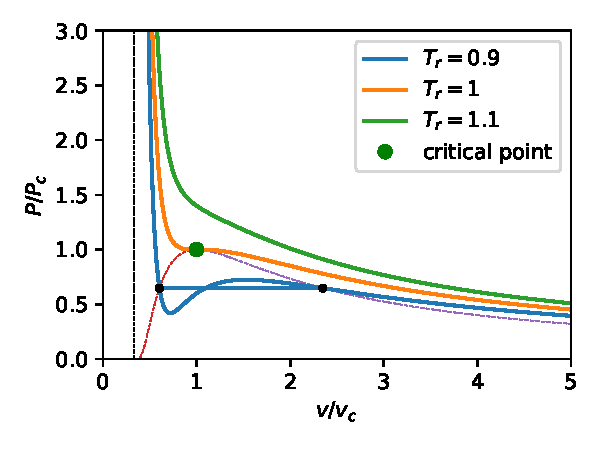
\includegraphics[scale=0.8]{figures/isotherms of the van der Waals gas.pdf}
		\caption{isotherms of the van der Waals gas.}
	\end{figure}
\end{itemize}

\subsection{critical exponents and fluctuations}
\begin{itemize}
	\item 根据 \eqref{10.2.13}, 在 critical point 附近, $T_r < 1$ 时, 有
	\begin{equation}
		v_{r, \text{liquid}} \simeq 1 - \frac{\Delta}{2}, \quad v_{r, \text{gas}} \simeq 1 + \frac{\Delta}{2},
	\end{equation}
	得到
	\begin{equation}
		T_r \simeq 1 - \frac{1}{16} (v_{r, \text{gas}} - v_{r, \text{liquid}})^2 \iff v_\text{gas} - v_\text{liquid} \sim (T_c - T)^{1 / 2}.
	\end{equation}
	
	\item 因为在 critical point $\big( \frac{\partial P}{\partial v} \big)_{T, N} = \big( \frac{\partial^2 P}{\partial v^2} \big)_{T, N} = 0$, 所以
	\begin{equation}
		P - P_c \sim (v - v_c)^3 \Longrightarrow \kappa_T = - \frac{1}{v} \Big( \frac{\partial v}{\partial P} \Big)_{T, N} \sim (T - T_c)^{- 1},
	\end{equation}
	可见, 在 critical point $\kappa_T \rightarrow \infty$, 根据 \eqref{4.4.2}, 直接后果就是
	\begin{equation}
		\braket{(\Delta N)^2} \rightarrow \infty.
	\end{equation}
\end{itemize}

\section{the Ising model}
\begin{itemize}
	\item 
\end{itemize}
